\documentclass[12pt,a4paper]{article}
%-----------------------PACKAGES-----------------------%
\usepackage[top=1in,bottom=1in,left=0.5in,right=0.5in]{geometry}
\usepackage{graphicx}
\usepackage{array}
\usepackage{xcolor}
\usepackage{adjustbox}
\usepackage{titlesec}
\usepackage{svg}
\usepackage{lettrine}
\usepackage{blindtext}
\usepackage{fancyhdr}
\usepackage{hyperref}
\hypersetup{
    colorlinks=true,
    linkcolor=violet,
    filecolor=magenta,      
    urlcolor=cyan,
    pdftitle={Overleaf Example},
    pdfpagemode=FullScreen,
    }


%-----------------------TABLES ALIGNEMNET-----------------------%

%-----------------------TITLE DOCUMENT-----------------------%
\begin{document}
\clearpage\thispagestyle{empty}
	\begin{Titlepage}
\begin{center}
    \vspace*{2cm}
    
    \textbf{\Huge Assignment\#}\\
    \vspace*{2cm}
    
      
      \vspace{0.2cm}
      \begin{center}
          \large M.Wahaj Tahir\\F191014@cfd.nu.edu.pk\\wahajt@acm.org
      \end{center} 
    
    \vspace{1.5cm}
    \begin{center}
    \large April,2023 
    \end{center}
    
    \vfill
    \vspace{0.8cm}
    \begin{figure}[hb]
        \centering
        \includegraphics[scale=0.20]{Fast-Nuces.png}
    \end{figure}
    Department of Computer Science\\ National University of Computer and Emerging Science\\ Chiniot Faisalabad Campus, Pakistan 2023
    \end{center}
\end{Titlepage}









 


 
 
 \clearpage
%-----------------------TABLE OF CONTENT-----------------------% 
\tableofcontents
\clearpage
%-----------------------TABLE OF CONTENT-----------------------% 

\section{Questions}
\subsection{How many weeks did you attend the internship}
\begin{itemize}
    \item I have attended 4 weeks.
\end{itemize}
\subsection{How many (approx) hours did you spend on all activities related to the internship}
\begin{itemize}
    \item I was giving 3-4 hours per day.
\end{itemize}
\subsection{What did you learn throughout the course of the internship}
\begin{itemize}
    \item This opportunity had opened door for me  to explore new domain in finance with programming which is something new to me as being a computer science background i never heard from my seniors that they ever worked in fiance,Overall this internship showed me a new path in trading which is worth it learning.
\end{itemize}
\subsection{What do you think can be improved in the Internship}
\begin{itemize}
    \item Assuming interns are new to python, I highly recommend using VS code.It has very good extensions and it also supports Jupyter Notebook.The extensions you install helps alot in debugging the issues.
\end{itemize}
\subsection{Based on the Stipend Table above please create a new table for yourself}
\begin{table}[h!]
    \centering
    \caption{Stipend Table }
    \begin{tabular}{|l|p{5cm}|}
        \hline
      Section 1 (Done) &\$25 \\ %end of row
       \hline %creating the row line at top
        Section 2 (Done) &\$40 \\ %end of row
       \hline %creating the row line at top
        Section 3 (Done) &\$50 \\ %end of row
       \hline %creating the row line at top
        Section 4 (Chapter 1-8)(Done) &Based on final project\\ %end of row
       \hline %creating the row line at top
        Section 5 (Final Project)(Done) &\$50-\$400 (\$50/chapter based on the number of chapters from the book used in the final project)\\ %end of row
       \hline %creating the row line at top 
       \textbf{Total}&\$380\\ %end of row
       \hline %creating the row line at top 
    \end{tabular}
\end{table}
% \textbf{Bank Name:} Allied Bank \\
% \textbf{Account Title:} Muhammad Wahaj Tahir\\
% \textbf{Account No:} 08700010064057290014\\
\clearpage
\textbf{Asana Board:}
\begin{figure}[h]
        \centering
        \includegraphics[scale=0.25]{SS/Asana.png}
              \caption{Asana Board}
    \end{figure} 
\clearpage
\section{Final Project}
I will give an overview of the project in sequence followed in the document.
\subsection{Download minute resolution data of NVDA for the past 60 days from Yahoo Finance}
\begin{itemize}
    \item When I tried to download minute resolution data it did throw me an error"Only 7 days worth of 1m granularity data are allowed to be fetched per request."
    \item For that I was only able to fetch 1-day data so I fetch past 200 days.
    \item For computing the SMA I used \textbf{Adj Close} column because it gives more accurate answers.
    \begin{figure}[h]
        \centering
        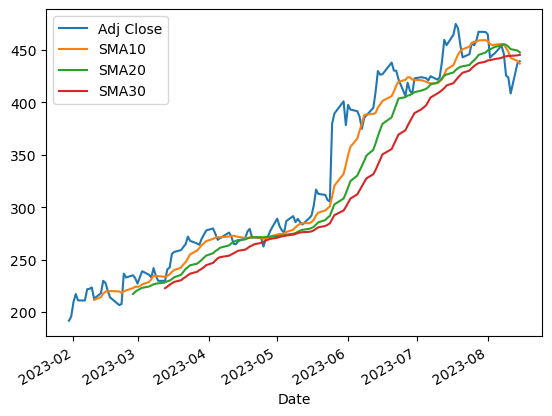
\includegraphics[scale=1]{Adj_SS/plot.png}
              \caption{SMA10,20,30}
    \end{figure} 
\end{itemize}
\clearpage
\subsection{Create a strategy\#1}
\begin{figure}[h]
        \centering
        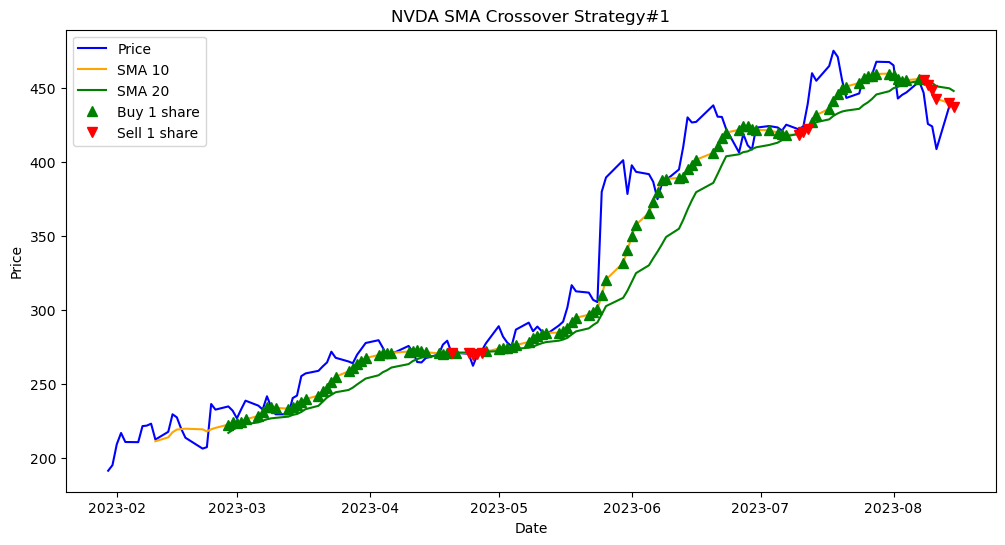
\includegraphics[scale=0.50]{Adj_SS/S1.png}
              \caption{Strategy\#1}
    \end{figure} 
\subsection{Create a strategy\#2}
\begin{figure}[h]
        \centering
        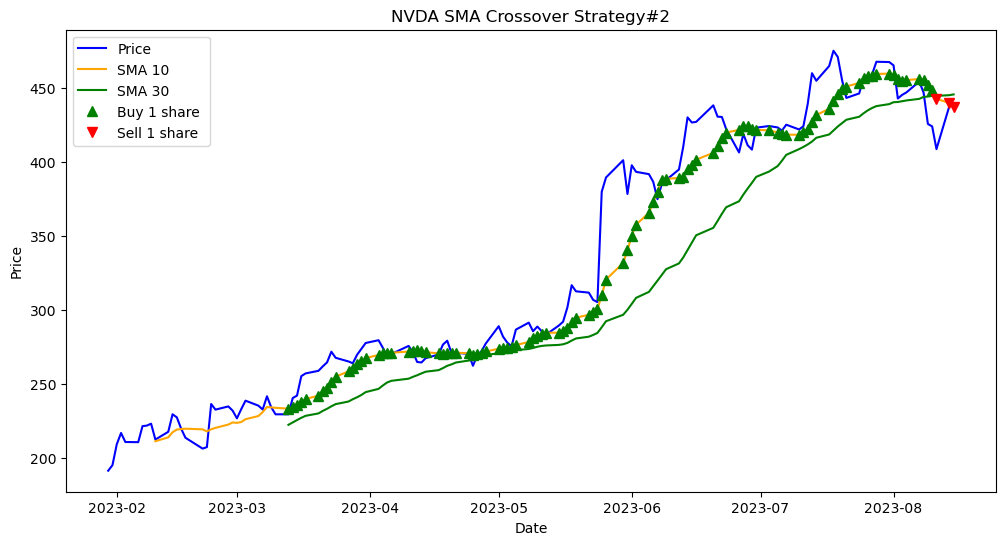
\includegraphics[scale=0.50]{Adj_SS/S2.png}
              \caption{Strategy\#2}
    \end{figure} 
\clearpage
\subsection{ performance metrics of strategies 1 and 2}
\begin{figure}[h]
        \centering
        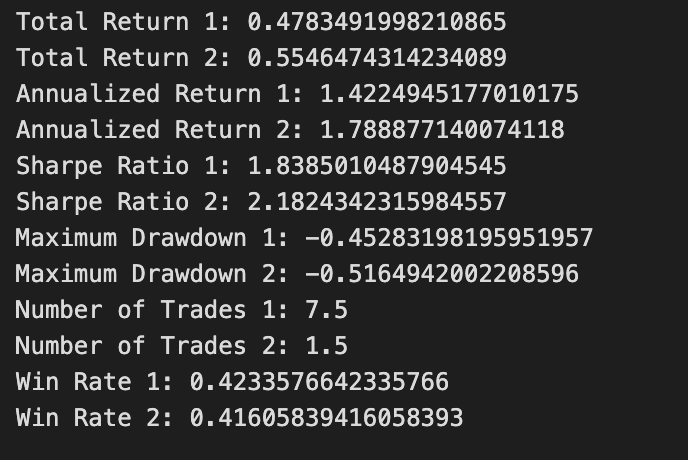
\includegraphics[scale=0.50]{Adj_SS/AdjPerfomrance.png}
              \caption{Performance Metrics}
    \end{figure}
    \begin{table}[h!]
    \centering
    \caption{Performance Metrics}
    \begin{tabular}{|l|p{9cm}|}
        \hline
      \textbf{Total Return}&Strategy 2 (0.5546) has a higher total return than Strategy 1 (0.4783), which suggests that Strategy 2 has generated more profit over the specified time period. \\ %end of row
       \hline %creating the row line at top
        \textbf{Annualized Return}&Strategy 2 (1.7889) also has a higher annualized return than Strategy 1 (1.4225). This means that, on average, Strategy 2 has produced greater returns per year compared to Strategy 1. \\ %end of row
       \hline %creating the row line at top
        \textbf{Sharpe Ratio}&Strategy 2 (2.1824) has a higher Sharpe ratio than Strategy 1 (1.8385), indicating that Strategy 2 has provided a better risk-adjusted return, considering the volatility of the returns. \\ %end of row
       \hline %creating the row line at top
        \textbf{Maximum Drawdown}&Both strategies have experienced drawdowns, with Strategy 2 having a slightly larger maximum drawdown (-0.5165) compared to Strategy 1 (-0.4528). A lower maximum drawdown is generally preferred, as it signifies a smaller decline from the peak portfolio value. \\ %end of row
       \hline %creating the row line at top
        \textbf{Number of Trades}&Strategy 1 (7.5) has a higher number of trades than Strategy 2 (1.5). This suggests that Strategy 1 is more active, potentially resulting in higher transaction costs and more frequent adjustments to the portfolio. \\ %end of row
       \hline %creating the row line at top
        \textbf{Win Rate}&Both strategies have relatively similar win rates, with Strategy 1 (0.4234) having a slightly higher win rate than Strategy 2 (0.4161). \\ %end of row
       \hline %creating the row line at top
    \end{tabular}
\end{table}
\clearpage
    \subsection{Evaluation of Strategy 1 and 2}
    \begin{figure}[h]
        \centering
        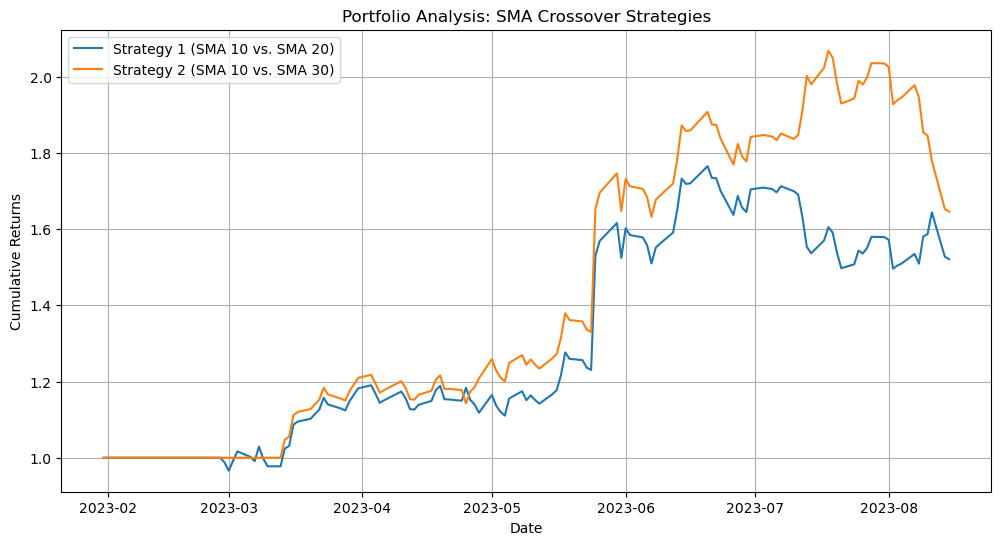
\includegraphics[scale=0.50]{Adj_SS/PortAnalysis.png}
              \caption{Comparing}
    \end{figure}
\textbf{Conclusion:}
\par{\newline Strategy 2 has performed better than Strategy 1 in terms of total return, annualized return, Sharpe ratio, and maximum draw down.
\par\newline However, it's important to consider the context, market conditions, and other relevant factors when making a decision. A higher return doesn't always imply a better strategy, especially if it comes with significantly higher risk or other limitations. It's advisable to analyze these metrics alongside other relevant information before making any investment decisions.}
\clearpage
\subsection{Create a table that describes what you learned from each chapter and how you applied it}
\begin{table}[h!]
    \centering
    \caption{Chapters Description }
    \begin{tabular}{|l|p{9cm}|}
        \hline
      \textbf{Chapter 1}&Inchapter 1 the author talked about the basic understanding of a book, how it is written, how to proceed with it, and how to keep the flow maintained.\ \\ %end of row
       \hline %creating the row line at top
       \textbf{Chapter 2}&The author has explained systematic approach why we need it,he talks about the methodology, time management,why do we need a model,How to perform back testing effectively etc. \\ %end of row
       \hline %creating the row line at top
      \textbf{Chapter 3}&The author talked about which parameters are essential in constructing a linear model. Moreover, he talks about rules,risk, and investment strategies. \\ %end of row
       \hline %creating the row line at top
       \textbf{Chapter 4}&Sharpe ratio for risk and adjusted its performance. \\ %end of row
       \hline %creating the row line at top
       \textbf{Chapter 5}&Performed backtesting using SMA crossover strategy using pandas.\\ %end of row
       \hline %creating the row line at top
       \textbf{Chapter 6}&Created graphs of prices,SMA10,20,30. \\ %end of row
       \hline %creating the row line at top
       \textbf{Chapter 7}&Didn't use zipline,but I have provided the solution to setup. \\ %end of row
       \hline %creating the row line at top
       \textbf{Chapter 8}&Returns, volatility, drawdowns, and other risk-related measures are showed in performance metrics. \\ %end of row
       \hline %creating the row line at top
    \end{tabular}
\end{table}

    

    

\end{document}